\documentclass[fleqn]{article}
\oddsidemargin 0.0in
\textwidth 6.0in
\thispagestyle{empty}
\usepackage{import}
\usepackage{amsmath}
\usepackage{graphicx}
\usepackage{flexisym}
\usepackage{amssymb}
\usepackage{bigints} 
\usepackage[english]{babel}
\usepackage[utf8x]{inputenc}
\usepackage{float}
\usepackage[colorinlistoftodos]{todonotes}

\definecolor{hwColor}{HTML}{AD53BA}

\begin{document}

  \begin{titlepage}

    \newcommand{\HRule}{\rule{\linewidth}{0.5mm}} % Defines a new command for the horizontal lines, change thickness here

    \center % Center everything on the page



    \textsc{\LARGE Arizona State University}\\[1.5cm] % Name of your university/college

    \textsc{\LARGE Mathematical Methods For Physics II }\\[1.5cm] % Major heading such as course name


    \begin{figure}
      
\includegraphics[width=\linewidth]{asu.png}
    \end{figure}


    \HRule \\[0.4cm]
    { \huge \bfseries Homework Nine}\\[0.4cm] 
    \HRule \\[1.5cm]

    \textbf{Behnam Amiri}

    \bigbreak

    \textbf{Prof: Cecilia Lunardini}

    \bigbreak


    \textbf{{\large \today}\\[2cm]}

    \vfill % Fill the rest of the page with whitespace

  \end{titlepage}

  \textbf{Part A}
  \begin{enumerate}

    \item  A heavy flexible chain of length $l$ and weight $w$ ($w=Mg$, with $M$ the mass of the string, and $g$ the acceleration of gravity) hangs vertically. The string has constant mass per unit length, $\mu$.  Its lower end is free to move. Consider the displacement $X(y,t)$ of the string with respect to its equilibrium position, where $y$ is a coordinate along the string, and $t$ is time. Set $y=0$ to coincide with the bottom of the chain.  
      \begin{enumerate}
        \item {\bf Bonus: } Newton's second law of dynamics, prove that $X(y,t)$ is described by the following differential equation: 
      \begin{equation}
      \frac{\partial}{\partial y}\left( y\frac{\partial X}{\partial y} \right) = \frac{1}{g} \frac{\partial^2 X}{\partial t^2}.
      \label{eq:chainEOM}
      \end{equation}
      
      
      (assume small oscillations, i.e., that each particle of the chain oscillates in a horizontal line. You will need to use some approximations involving trigonometric functions, similarly to what is usually done for the problem of a horizontal vibrating string) 
      
        \textcolor{hwColor}{
          \\
          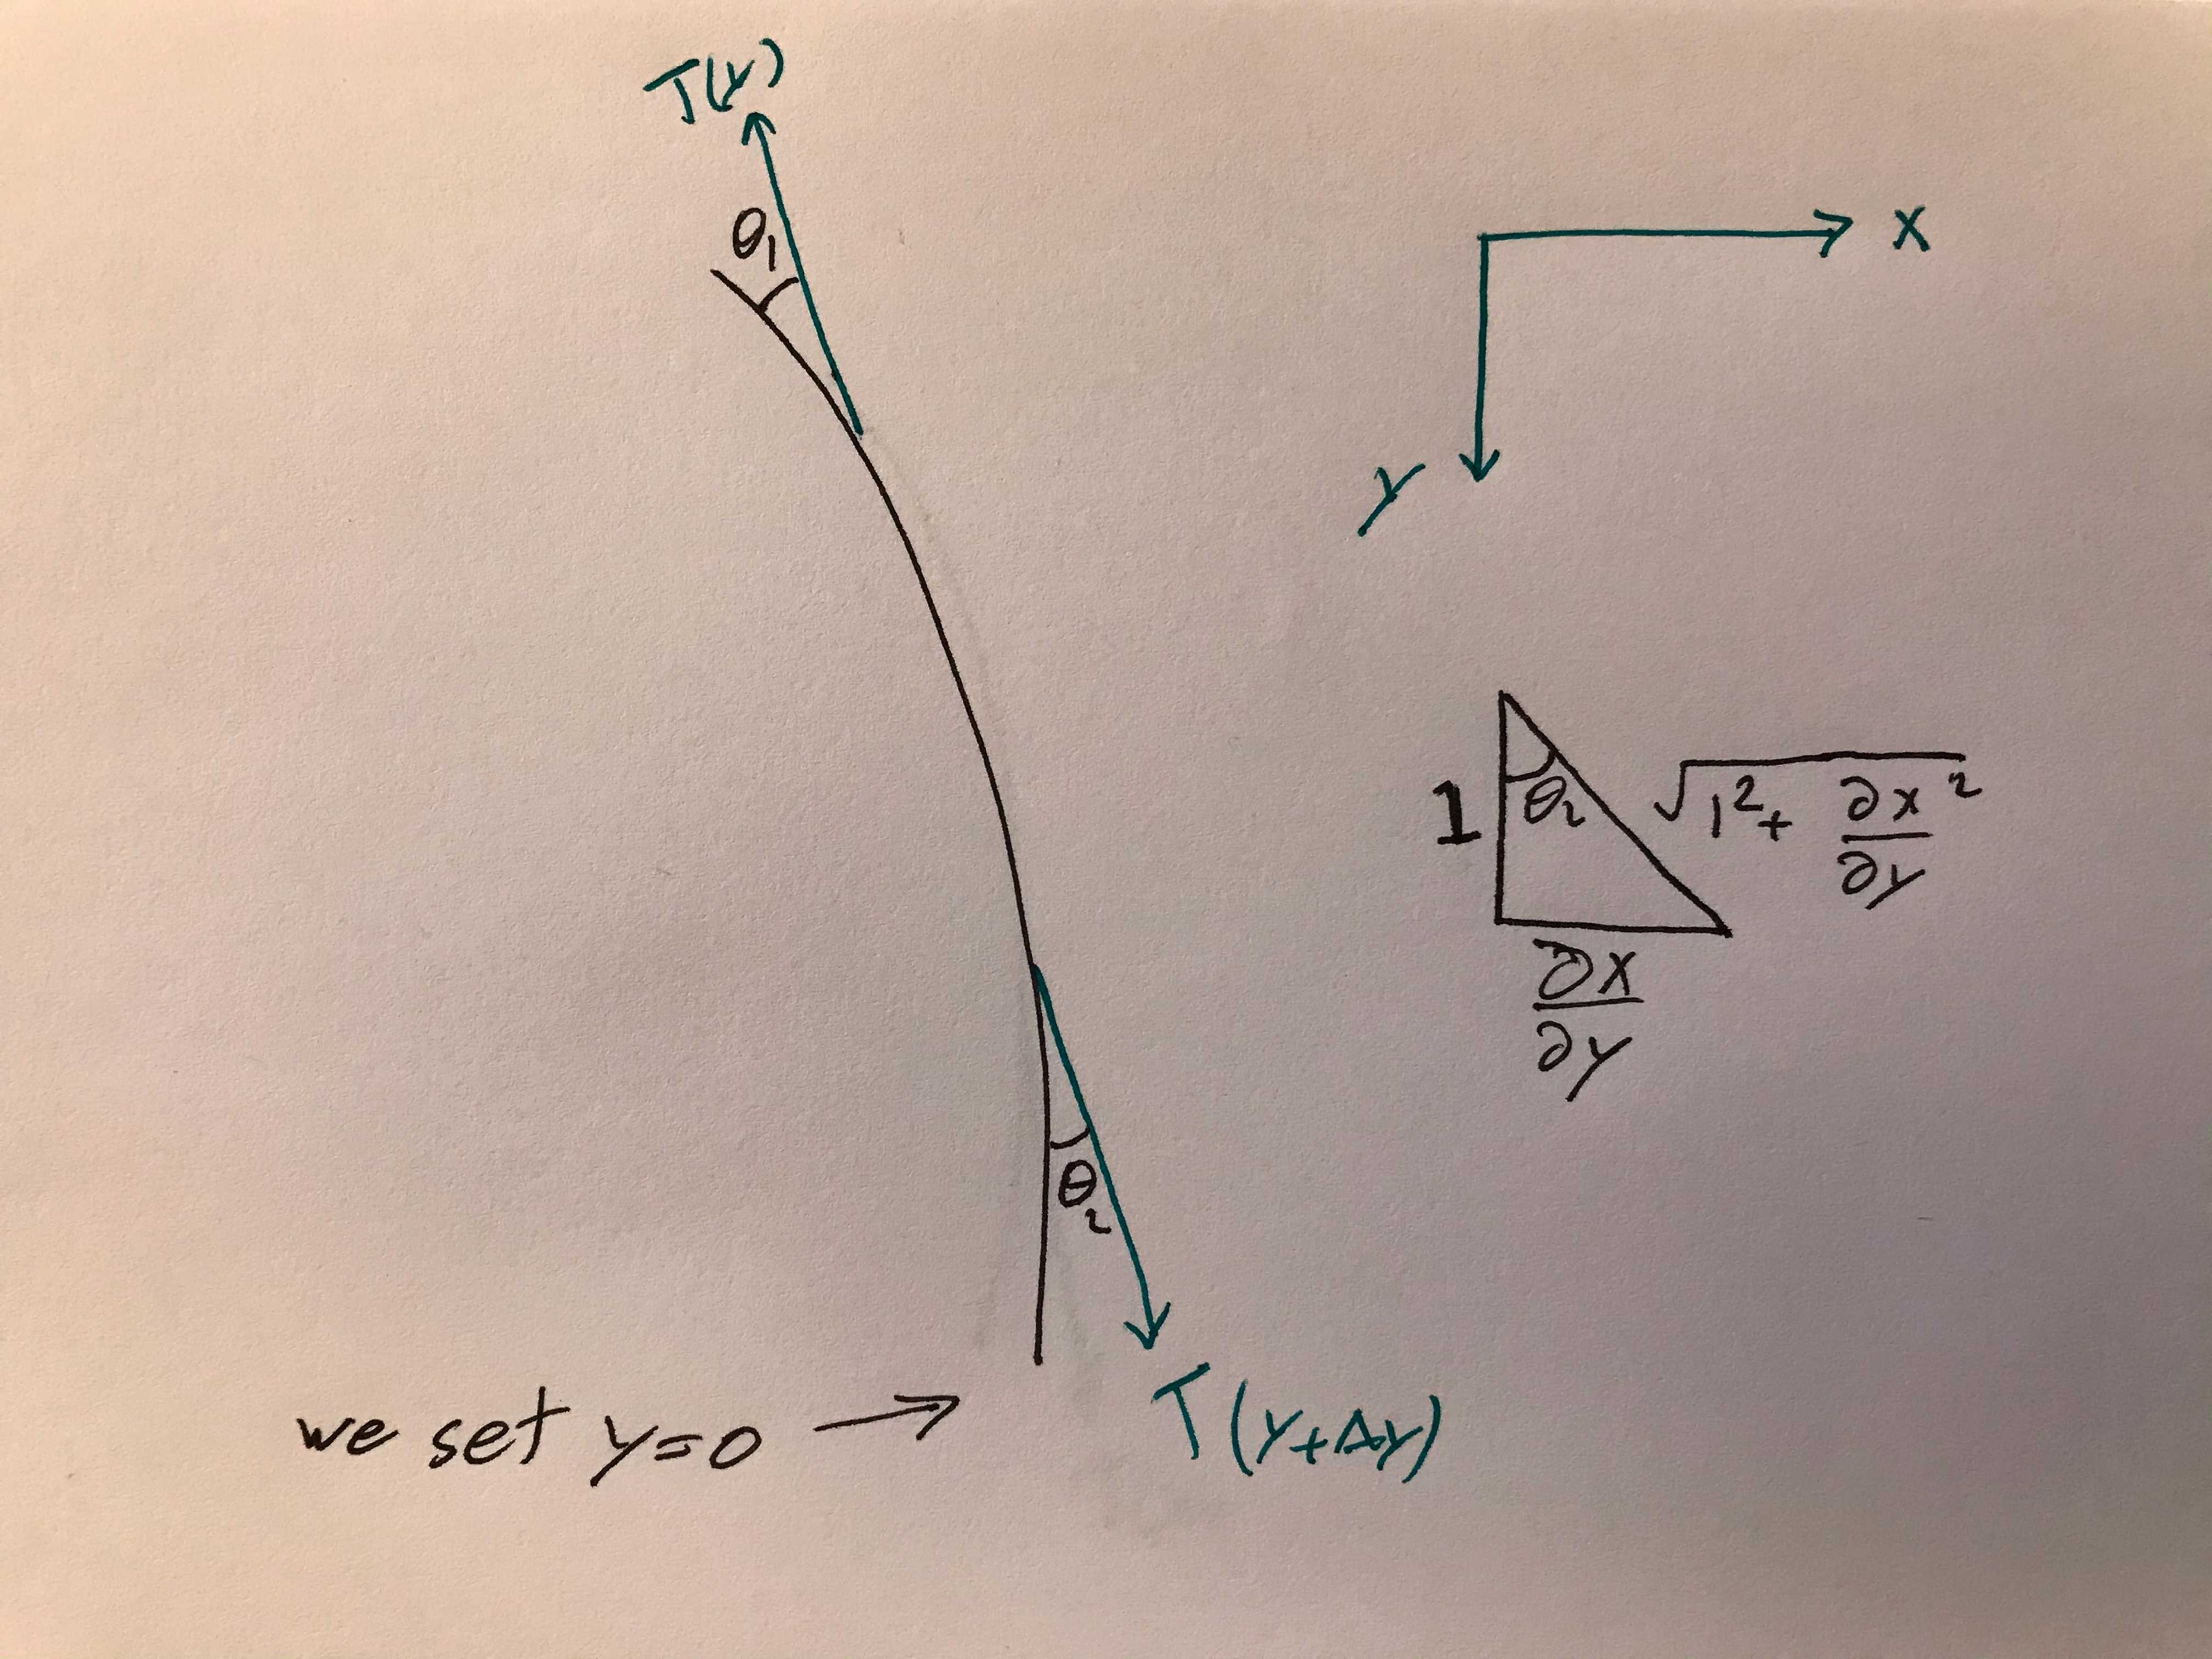
\includegraphics[height=5cm, width=9cm]{one.jpg}
          \\
          In order to derive the equation of motion, we will invoke Newton’s second law, which states that
          the sum of the forces acting on a body is equal to its mass times its acceleration. Mathematically
          this is written as 
          $$\sum \mathbf{F}=m\mathbf{a}$$ \\
          \\
          For this problem we will choose the coordinate system as shown in the figure, 
          so there are two equations of significance. \\
          \\
          $$\sum \mathbf{F}_x=m\mathbf{a}_x$$ \\
          $$\sum \mathbf{F}_y=m\mathbf{a}_y$$ 
          \\
          We got two forces acting on this chain, $\mathbf{T}$ at $y$ and $\mathbf{T}$ 
          at $y+\Delta y$.
          The motion of the chain is entirely in the x-direction, which means there is no vertical component of acceleration
          $(a_y=0)$.
          \\
          \\
          \textbf{Y-Direction:} \\ \\
          $
            \mathbf{F}_y=m\mathbf{a}_y=-T(y) cos(\theta_y)+T(y+\Delta y) cos(\theta_{y+\Delta y})=0 \\
            \\
            =-T(y) \dfrac{1}{\sqrt{1^2+(\dfrac{\partial X}{\partial y})^2}}+T(y+\Delta y)\dfrac{1}{\sqrt{1^2+(\dfrac{\partial X}{\partial y})^2}}=0 \\
            \\
            \\
            T(y) \dfrac{1}{\sqrt{1^2+(\dfrac{\partial X}{\partial y})^2}}=T(y+\Delta y)\dfrac{1}{\sqrt{1^2+(\dfrac{\partial X}{\partial y})^2}} \\ \\
          $
          \textbf{Note:} Since we are considering an infinitesimal element of the chain, the two angles are pretty small, hence 
          $\theta_{y+\Delta y} \approx \theta_y =\theta$. \\
          \\
          $
            \therefore ~~~ T(y) \dfrac{1}{\sqrt{1^2+(\dfrac{\partial X}{\partial y})^2}}=T(y+\Delta y)\dfrac{1}{\sqrt{1^2+(\dfrac{\partial X}{\partial y})^2}} ~~~ \surd
          $
          \\
          \\
          \rule{15cm}{1pt}
          \\
          \\
          \textbf{X-Direction:} \\ \\
          $
            \mathbf{F}_x=m\mathbf{a}_x=-T(y) sin(\theta)+T(y+\Delta y) sin(\theta) \\
            \\
            =-T(y) \dfrac{\dfrac{\partial X}{\partial y}}{\sqrt{1^2+(\dfrac{\partial X}{\partial y})^2}}+T(y+\Delta y)  \dfrac{\dfrac{\partial X}{\partial y}}{\sqrt{1^2+(\dfrac{\partial X}{\partial y})^2}}=m a_x \\
            \\
          $
          \\
          Understand that $a_x=\dfrac{\partial^2 X}{\partial t^2}$ the acceleration at a specific point on the chain at time $t$. 
          To get the force we therefore have to multiply it by a tiny bit of mass $\Delta m$. As we know mass is density times
          length, so this can be written in terms of arc length, $s$, as $\Delta m=\mu \Delta s$. Newton’s second law in the X-Direction is thus: \\
          \\
          $
            -T(y) \dfrac{\dfrac{\partial X}{\partial y}}{\sqrt{1^2+(\dfrac{\partial X}{\partial y})^2}}+T(y+\Delta y)  \dfrac{\dfrac{\partial X}{\partial y}}{\sqrt{1^2+(\dfrac{\partial X}{\partial y})^2}}=\bigints dm \dfrac{\partial^2 X}{\partial t^2}=\bigints \mu ds \dfrac{\partial^2 X}{\partial t^2} \\
            \\
          $
          \\
          \textbf{Attention:} $\sqrt{1^2+(\dfrac{\partial X}{\partial y})^2} \approx 1$ since $\dfrac{\partial X}{\partial y}$ is the
          the slope of an infinitesimal displacement. This allows us to simplify the above equation as:\\
          \\
          \\
          $
            -T(y) \dfrac{\partial X}{\partial y}+T(y+\Delta y) \dfrac{\partial X}{\partial y}=\bigints \mu ds \dfrac{\partial^2 X}{\partial t^2} \\
            \\
          $
          Based on our assumption for this problem, the tension on the chain depends on the mass of the chain. We can integrate the length 
          of chain with respect to its mass per unit length to find its mass and then if we multiple the result by gravity, We 
          end up getting the weight: \\
          \\
          $$T(y)=\bigints_{0}^{y} \sqrt{1^2+(\dfrac{\partial X}{\partial y}})^2 \mu g=y \mu g$$ \\
          \\
          \\
          $
            \bigints \dfrac{\partial }{\partial y} \left(T \dfrac{\partial X}{\partial y} \right) dy=\bigints \mu ds \dfrac{\partial^2 X}{\partial t^2}=\dfrac{\partial^2 X}{\partial t^2} \mu \bigints  \sqrt{1^2+(\dfrac{\partial X}{\partial y}})^2  dy=\dfrac{\partial^2 X}{\partial t^2} \mu \bigints dy \\ \\
            \\
            \bigints \dfrac{\partial }{\partial y} \left(T \dfrac{\partial X}{\partial y} \right) dy=\dfrac{\partial^2 X}{\partial t^2} \mu \bigints dy \\
            \\
            \\
            \dfrac{\partial }{\partial y} \left(y \mu g \dfrac{\partial X}{\partial y} \right)=\dfrac{\partial^2 X}{\partial t^2} \mu 
            \Rightarrow \mu g  \dfrac{\partial }{\partial y} \left(y\dfrac{\partial X}{\partial y} \right)=\dfrac{\partial^2 X}{\partial t^2} \mu
            \\
            \\
            \\
            \\
            \therefore ~~~~ \dfrac{\partial }{\partial y} \left(y\dfrac{\partial X}{\partial y} \right)=\dfrac{1}{g}\dfrac{\partial^2 X}{\partial t^2} ~~~ \surd
          $
        }

      \item Using the method of the separation of the variables, find the general solution of the equation above.  Using the method illustrated in class 16, 
      show that the general solution involves Bessel functions. Find the chain's natural frequencies of oscillation.
      
      
        \textcolor{hwColor}{
          \\
          The method of separation of variables relies upon the assumption that a function of the form
          $u(x,y)=\Phi(x)Y(y)$, will be a solution to a linear homogeneous partial differential equation in $x$
          and $y$. This is called a product solution and provided the boundary conditions are also linear and
          homogeneous this will also satisfy the boundary conditions. The method of Separation of Variables
          cannot always be used and even when it can be used it will not always be possible to get much past
          the first step in the method. \\
          \\
          This is what we found in section \textbf{(a)}. We guess that a potential solution is $X(y,t)=Y(y)\Phi(t)$. Hence, \\
          \\
          $
            \dfrac{\partial }{\partial y} \left(y\dfrac{\partial X}{\partial y} \right)=\dfrac{1}{g}\dfrac{\partial^2 X}{\partial t^2}
            \Rightarrow \dfrac{\partial X}{\partial y}+y\dfrac{\partial^2 X}{\partial y^2}=\dfrac{1}{g}\dfrac{\partial^2 X}{\partial t^2} 
            \\
            \\
            \dfrac{\partial}{\partial y}\left[Y(y)\Phi(t)\right]+y\dfrac{\partial^2}{\partial y^2} \left[Y(y)\Phi(t)\right]=\dfrac{1}{g}\dfrac{\partial^2}{\partial t^2} \left[Y(y)\Phi(t)\right] \\
            \\
            \\
            \Phi(t) \dfrac{\partial}{\partial y}\left[Y(y)\right]+y\Phi(t) \dfrac{\partial^2}{\partial y^2} \left[Y(y)\right]=\dfrac{Y(y)}{g}\dfrac{\partial^2}{\partial t^2} \left[\Phi(t)\right] \\
            \\
            \\
          $
          To make our work easier, let's use some alias: \\
          \\
          $
            \begin{cases}
              \dfrac{\partial}{\partial y}\left[Y(y)\right]=Y_y \\
              \\
              \dfrac{\partial^2}{\partial y^2} \left[Y(y)\right]=Y_{yy} \\
              \\
              \dfrac{\partial^2}{\partial t^2} \left[\Phi(t)\right]=\Phi_{tt}
            \end{cases} \\
            \\
            \\
            \Phi Y_y+y\Phi Y_{yy}=\dfrac{Y}{g}\Phi_{tt} \Rightarrow
            \dfrac{\Phi Y_y+y\Phi Y_{yy}}{Y \Phi}=\dfrac{\dfrac{Y}{g}\Phi_{tt}}{Y \Phi}
            \Rightarrow \dfrac{Y_y}{Y}+\dfrac{y}{Y} Y_{yy}=\dfrac{1}{g} \dfrac{\Phi_{tt}}{\Phi} \\ \\ \\
          $
          \rule{15cm}{1pt} \\
          \\
          \textbf{R.H.S:} \\ \\
          If $\dfrac{1}{g} \dfrac{\Phi_{tt}}{\Phi}=-\alpha^2$, then $\Phi_{tt}+g \alpha^2 \Phi=0$. \\
          \\
          \\
          $
            \therefore ~~~ \Phi=Acos\left[\alpha \sqrt{g}t\right]+B sin\left[\alpha \sqrt{g}t\right]
          $ \\
          \\
          \rule{15cm}{1pt} \\
          \\
          \textbf{L.H.S:} \\ \\
          $
            \dfrac{Y_y}{Y}+\dfrac{y}{Y} Y_{yy}=-\alpha^2 \Rightarrow yY_{yy}+Y_y+\alpha^2 Y=0 \Rightarrow y^2 Y_{yy}+y Y_y+y \alpha^2 Y=0 \\ \\
            \\
            \\
          $
          So far so Nooice, now it is time to \textbf{transform our second-order differential equation into a Bessel’s equation}. \\ \\
          \\
          \\
          \textbf{A quick review:} \\
          \\
          The Bessel functions of the second kind, denoted by $Y_{\alpha}(x)$, are solutions of 
          the Bessel differential equation that have a singularity at the origin $(x = 0)$ and are multivalued.
          For a Bessel’s equation like this $$u^2 \dfrac{d^2 f}{du^2}+u\dfrac{df}{du}+\left(u^2-m^2\right)=0$$
          When $u=Kx^{\beta}, ~~ y(x)=x^{\alpha} f(u)$, we have:
          $$x^2 \dfrac{d^2 y}{dx^2}+(1-2\alpha)x\dfrac{dy}{dx}+\left[\alpha^2 +\beta^2\left(C^2 x^{2\beta}-m^2\right)\right]y=0$$
          \\
          \\
          This equation gives us three parameters ($\alpha$, $\beta$, and $C$) that we can use to transform our
          second-order differential equations. the goal is to transform the given differntial equation into
          a Bessel’s equation form. \\
          \\
          $
            \begin{cases}
              y^2 Y_{yy}+y Y_y+y \alpha^2 Y=0 \\
              \\
              y^2 Y^{''}+\left(1-2a\right)y Y^{'}+\left[a^2+b^2\left(C^2 y^{2b}-m^2\right)\right]Y=0
            \end{cases} \Longrightarrow \begin{cases}
              a=0 \\
              \\
              m=0 \\
              \\
              b=\dfrac{1}{2} \\
              \\
              C=2 \alpha
            \end{cases} \\
            \\
            \\
          $
          So we can write the solution as: \\
          \\
          $
            Y(y)=W Y_1(y)+M Y_2(y)=W y^0 \mathcal{J}_m(cy^b) +M y^0 \mathcal{Y}_m(cy^b) \\
            \\
            \\
            \therefore ~~~ Y(y)=W \mathcal{J}_0(2 \alpha \sqrt{y}) +M \mathcal{Y}_0(2 \alpha \sqrt{y})
          $
          \\
          \rule{15cm}{1pt} \\
          \\
          Alright, time to wrap up what have found so far: \\
          \\
          $
            X(y,t)=Y(y)\Phi(t)=\left[W \mathcal{J}_0(2 \alpha \sqrt{y}) +M \mathcal{Y}_0(2 \alpha \sqrt{y})\right] \times \left[Acos\left[\alpha \sqrt{g}t\right]+B sin\left[\alpha \sqrt{g}t\right]\right] \\
            \\
            =\mathcal{J}_0(2 \alpha \sqrt{y}) Acos\left[\alpha \sqrt{g}t\right]+B sin\left[\alpha \sqrt{g}t\right] \\
            \\
            \\
          $
          \\
          \\
          Our final solution is: \\
          \\
          \\
          $
            \therefore ~~~~ \sum\limits_{n=0}^{\infty} \mathcal{J}_0(2 \alpha_n \sqrt{y}) A_n cos\left[\alpha_n \sqrt{g}t\right]+B_n sin\left[\alpha_n \sqrt{g}t\right]
          $
        }

    \end{enumerate}
    
    
  \end{enumerate}


  \textbf{Part B}
  \begin{enumerate}
    \item Derive the equation at the top of page 578 of the textbook (non-numbered equation immediately before eq. (18.2)). 
    
      \textcolor{hwColor}{
        We are asked to derive the following equation
        $$\sum\limits_{n=0}^{\infty} \{(n+2)(n+1)a_{n+2} -\left[n(n+1)-\ell (\ell+1)\right]a_n\}x^n=0$$ 
        The Legendre differential equation is the second-order ordinary differential equation
        $$(1-x^2)\dfrac{d^2 y}{dx^2}-2x\dfrac{dy}{dx}+\ell(\ell+1)y=0$$
        The Legendre differential equation can be solved using the Frobenius method by making 
        a series expansion with $k=0$: \\
        \\
        $
          y=\sum\limits_{n=0}^{\infty}a_n x^n
        $
        Plugging in, \\
        \\
        $
          (1-x^2)\dfrac{d^2 }{dx^2}\left[\sum\limits_{n=0}^{\infty}a_n x^n\right]-2x\dfrac{d}{dx}\left[\sum\limits_{n=0}^{\infty}a_n x^n\right]+\ell(\ell+1)\left[\sum\limits_{n=0}^{\infty}a_n x^n\right]=0 \\
          \\
          \\
          a_n(1-x^2)\dfrac{d^2 }{dx^2}\sum\limits_{n=0}^{\infty} x^n-2x a_n\dfrac{d}{dx}\sum\limits_{n=0}^{\infty} x^n+a_n\ell(\ell+1)\sum\limits_{n=0}^{\infty} x^n=0 \\
          \\
          \\
          \sum\limits_{n=0}^{\infty}\left[a_n(1-x^2)\dfrac{d^2 }{dx^2} x^n-2x a_n\dfrac{d}{dx} x^n+a_n\ell(\ell+1) x^n\right]=0 \\
          \\
          \\
          \sum\limits_{n=0}^{\infty}\left[a_n(1-x^2) n(n-1)x^{n-2}-2x a_n nx^{n-1}+a_n\ell(\ell+1) x^n\right]=0 \\
          \\
          \\
          \sum\limits_{n=0}^{\infty}\left[n(n-1)a_n x^{n-2}-x^2n(n-1)a_n x^{n-2}-2na_nx^n+a_n\ell(\ell+1) x^n\right]=0 \\
          \\
          \\
          \sum\limits_{n=0}^{\infty}\left[n(n-1)a_nx^{n-2}+a_nx^n\left(\ell(\ell+1)-n(n-1)-2n\right)\right]=0 \\
          \\
          \\
          \sum\limits_{n=0}^{\infty} \left[(n+1)(n+2)a_{n+2}x^n+a_n x^n \left(\ell(\ell+1)+n-n^2-2n\right)\right] \\
          \\
          \\
          \\
          \therefore ~~~ \sum\limits_{n=0}^{\infty} x^n\{(n+1)(n+2)a_{n+2} -\left[n(n+1)-\ell (\ell+1)\right]a_n\}=0 ~~~ \surd
        $
      }

    \item Starting from the expression of the Legendre equation, compute its Wronskian (see textbook, sec. 16.1 for a refresher on the Wronskian). Discuss the value(s) of $x$ for which the solutions to Legendre's equation may be undefined (hint: what values of $x$ are problematic for the Wronskian function?).
    
    
    \item Compute the Wronskians for the pairs, $P_0$ and $Q_0$, and $P_1$ and $Q_1$ (their expressions are given in the textbook). Are they what you expected?
    
    
    \item Consider the orthogonality property of Legendre Polynomials, eq. (18.12). Verify it explicitly (by direct computation) for the pairs $(P_2,P_3 )$ and $(P_2,P_4)$. 
    
  \end{enumerate}

\end{document}
